\documentclass[a4paper]{article}
\author{Alex}
\title{Problem Solving HW 16}
\usepackage{clrscode3e}
\usepackage{geometry}
\usepackage{tikz}
\usetikzlibrary{arrows}
\usepackage{amsmath,amssymb}
\usepackage{pst-blur}
\geometry{left = 2.0cm,right=2.0cm}
\begin{document}
\maketitle
\section*{22.1-3}
\subsection*{Use adjacency-list representation}
\begin{codebox}
\Procname{$\proc{graph-transpose(G)}$}
\li Let $G^T$ be a new graph with all vertices in G.
\li \For each $v \in G$ 
\li 	\Do \For each $u \in G.adj[v]$
\li		\Do add $v$ to $G^T.adj[u]$
		\End
	\End 
\li \Return $G^T$
\end{codebox}
Running Time $O(V+E)$
\subsection* {Use adjacency-matrix representation}
\begin{codebox}
\Procname{$\proc{graph-transpose(G)}$}
\li \For $i = 1$  \To $G.degree - 1$
\Do
\li \For $j = 0$ \To $i - 1$
\Do
\li exchange G[i][j] with G[j][i]
\End 
\End
\li \Return G
\end{codebox}
Running Time $O(V^2)$
\section*{22.1-8}
Suppose the hash table is implemented by linked list. If all the edges is hashed uniformly
then the expected time to decide whether an edge is in the graph is $O(1+\alpha)$, where $\alpha$ is the time to compute the hash hash function.
One big disadvantage is that it takes a lot of time to find all the vertices that are connected with a given vertex. Because you have to go through all the hash table or you need to check all other possible vertices. And like
adjacency-list, it takes a lot of time to remove a vertex. We can change Adj[\id{u}] to a dynamic array. All the verices in it is sorted. So we can use binary search to find an edge. And we can all decide all the vertices that are adjacent to a given vertex. But
it also takes a lot of time to remove or add a vertex. 
\section*{22.2-3}
Because only line 2 and 13 checks the color of a vertex, and both of the statements check whether a vertex is white or not, any color other than white will give the same result. More precisely, a vertex will only enter the queue once, so after a vertex had already entered the queue, no matter it has come out or not it won't enter the queue again. So there is no need for we to color a vertex black after it dequed.
\section*{22.2-4}
\begin{codebox}
\Procname {$\proc{BFS(G,s)}$}
\li \For each vertex $u \in G.V - \{s\}$
\li \Do \id{u.color} = \const{WHITE}
\li \id{u.d} = $\infty$
\li \id{u.\pi} = \const{NIL} \End
\li \id{s.color} = \const{GRAY}
\li \id{s.d} = 0
\li \id{s.\pi} = \const{NIL}
\li \id{Q} = $\emptyset$
\li \func {ENQUEUE(\id{Q,s})}
\li \While \id{Q} $\not=\emptyset$
\li \Do \id{u} = \func{DEQUEUE(\id{Q})}
\li \For \id{v} = 0 \To \id{G.degree}-1
\li     \Do \If \id{G[u][v]} == 1 AND \id{v.color} == \const{WHITE}
\li             \Do \id{v.color} = \const{GRAY}
\li             \id{v.d} = \id{u.d} + 1
\li             \id{v.\pi} = \id{u}
\li             \func{ENQUEUE(\id{Q,v})} \End\End\End
\end{codebox}
Running Time $O(V^2)$
\section*{22.2-5}
Since \id{u.d} = d(\id{s,v}), the distance between two  is independent from the way the graph is presented, so \id{u.d} is in dependent from the order in the adjacency-list.\\
 In Figure 22.3, if the adjacency-list of \id{w} is \id{\{x,t\}} rather than \id{\{t,x\}}, then \id{x} will enter the queue first thus makes \id{xu} be an edge in the breadth-first tree.
 \section*{22.3-6}
 The theorem 22.10 has already showed that there are only tree edges and back edges in a DFS of graph G. So we only need to show that for an edge (\id{u,v}) if (\id{u,v}) is encountered first then (\id{u,v}) is a tree edge otherwise it is a back edge.  (we must assume that \id{u} is discovered first, otherwise there is no difference between (\id{u,v}) and (\id{v,u})) So if (\id{u,v}) is discovered first, \id{v} must be white at that time. Because \id{v} is pushed into the stack after \id{u}, so when we are discovering \id{u}, \id{v} can't be in the stack, so it is either black or white. But if it is black then (\id{v,u}) must be already discovered. So \id{v} is white then (\id{u,v})  is a tree edge. As mentioned above while discovering (\id{u,v}), \id{v} can be either white or black, so if it is black, then (\id{v,u}) is first discovered, and when (\id{v,u}) is discovered, \id{u} is gray, so (\id{v,u}) is a back edge.
 \section*{22.3-7}
 To do this, an extra pointer is needed for all the vertices which points to the next vertices to discover, this pointer is set to the first element of the adjacency-list of each vertex at first.\\
 We only need to change DFS-VISIT.
 \begin{codebox}
 \Procname{$\proc{DFS-VISIT(G)}$}
 \li \id{time} = \id{time} + 1
 \li \id{u.d} = \id{time}
 \li \id{u.color} = \const{GRAY}
 \li \func{PUSH(\id{S,u})}
  \li \While \id{S} $\not= \emptyset$
  \li \Do \id{t} = \id{S.top}
  \li 	\If \id{t.p} == \const{NIL} 
  \li 		\Do \id{time} = \id{time} + 1
  \li			\id{t.f} = \id{time}
  \li			\id{t.color} = \const{BLACK}
  \li			\func{POP(\id{S})} 
  \li	\Else 
  \li 		\If \id{t.p.color} == \const{WHITE}
  \li		\Do  \id{time} = \id{time} + 1
  \li			\id{t.p.d} = \id{time}
  \li			\id{t.p.color} = \const{GRAY}
  \li			\func{PUSH(\id{S,t.p})}  \End
  \li		Set \id{t.p} to the next vertex in the adjacency-list of t. \End
  \End
 \end{codebox}
 \section*{22.3-8}

 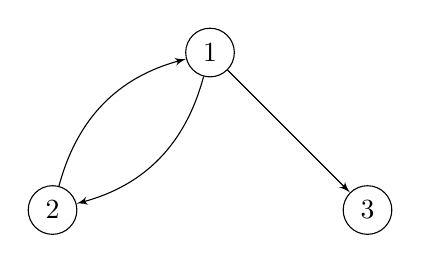
\begin{tikzpicture}
 \tikzset{vertex/.style = {shape=circle,draw,minimum size=1.5em}}
 \tikzset{edge/.style = {->,> = latex'}}
 \node[vertex] (a) at (0,0){2};
 \node[vertex] (b) at  (2,2) {1};
 \node[vertex] (c) at (4,0) {3};
 \draw[edge] (b) to [bend left] (a);
 \draw[edge] (a) to [bend left] (b);
 \draw[edge] (b) to (c);

 \end{tikzpicture}\\
 In this case, if we begin the DFS at 1, then \id{2.d} $<$ \id{3.d}
. But the forest it produces is:\\

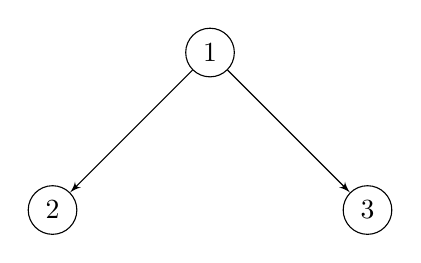
\begin{tikzpicture}
 \tikzset{vertex/.style = {shape=circle,draw,minimum size=1.5em}}
 \tikzset{edge/.style = {->,> = latex'}}
 \node[vertex] (a) at (0,0){2};
 \node[vertex] (b) at  (2,2) {1};
 \node[vertex] (c) at (4,0) {3};
 \draw[edge] (b) to (a);
 \draw[edge] (b) to (c);

 \end{tikzpicture}\\
 Obviously \id{3} is not \id{2}'s descendant.
 \section*{22.3-9}
 Use the same graph above. \id{2.f} = 3, \id{3.d} = 5,
  \id{2.f} $<$ \id{3.d}.

\section*{22.4-2}
We can use dynamic programming to solve this problem. Let
D(\id{u,t}) to be the number of simple paths between from
\id{u} to \id{t}. Then we have the transfer formula:\\
$$D(\id{u,t}) =
\begin{cases}
1& \id{u = t} \\
\sum_{v\in Adj[\id{u}]} D(\id{v,t})& \id{u \not= t}

\end{cases}$$
So it is pretty easy to design a top-town approach to solve
this problem. Since there are \id{V} subproblems and the number
of sub-subproblems equals to the outdgree of the corresponding
vertex. So the running time is $O(E)$ .
\section*{22.4-3}
Just simply modify the code for BFS. If we discovered any vertices that
is not white, then we can concluded there is a cycle. As for the
running time, if a graph contains no cycle, then there are at most
\id{|V|-1} edges, so the running time is $O(\id{V})$. And if a graph
contains a cycle, then it will explore at most \id{|V|-1} edges so the
running time is still $O(\id{V})$.
\section*{22.5-5}
First compute the strongly connected component of \id{G}. This would
take $O(\id{V}+\id{E})$ of time. Then for each tree we produced, we assign
a number for each vertex as the number of vertex in the $G^{SCC}$, this would take $O(\id{V}+\id{E})$ of time. Then we
go through all the edges. If the two vertices are in different tree, add them to
the $E(G^{SCC})$, this only takes $O(E)$ of time. From Lemma 22.13, we know it is impossible for two vertices have more than one edge.
So the time complexity of this algorithm is $O(V+E)$.
\section*{22.5-7}
First compute the component graph of \id{G}. Then we apply topological sort to $\id{G^{SCC}}$.
Then we get a linked list of strongly connected component. Then for every two adjacent vertices in the list,
check whether all of them are directly connected. If so this graph is semiconnected, otherwise it isn't.
\subsection*{Proof}
Obviously a graph \id{G} is semiconnected if and only if $\id{G^{SCC}}$ is semiconnected. (I want to skip the proof of this, it's too obvious.)
Since $\id{G^{SCC}}$ is a dag, we can apply topological sort to it. If every two adjacent vertices are directly connected, then it is semiconnected. But if
there exists two adjacent that are not directly connected, say \id{u} and \id{v}, and suppose \id{u} is before \id{v}. From the property of the topological sort,
we know that a vertex can only be directly connected with the vertices after it. So for \id{v} it can only be directly connected with the vertices after it, and none of them are connected directly with
\id{u}, so there isn't a \id{(v,u)} path. And for \id{u}, it only be connected with vertices after \id{v} and also none of them are directly connected to \id{v}. So there isn't a \id{(u,v)} path. So this graph is
not semiconnected, thus we finished the proof.\\
The time complexity is \id{O(V+E)}.

\end{document}
